%!TEX TS-options = --shell-escape
%!TEX TS-program = pdflatex
\documentclass[%
10pt,              % Schriftgroesse
ngerman,           % wird an andere Pakete weitergereicht
a4paper,           % Seitengroesse
DIV11,             % Textbereichsgroesse (siehe Koma Skript Dokumentation !)
]{scrartcl}%     Klassen: scrartcl, scrreprt, scrbook, article
% -------------------------------------------------------------------------

\usepackage[utf8]{inputenc} % Font Encoding, benoetigt fuer Umlaute
\usepackage[ngerman]{babel}   % Spracheinstellung

\usepackage[T1]{fontenc} % T1 Schrift Encoding
\usepackage{textcomp}    % Zusatzliche Symbole (Text Companion font extension)
\usepackage{lmodern,dsfont}     % Latin Modern Schrift
\usepackage{dsfont}
%\usepackage{wasysym}
\usepackage{ulem}
\usepackage{graphicx}
\usepackage{eurosym}
%\usepackage{txfonts}
\usepackage{stmaryrd}
\usepackage{amsfonts}
\usepackage{amsmath}
\usepackage{gensymb}
\usepackage{hyperref}
\usepackage{tikz}
\usepackage{multirow}
\usepackage{listings}
\usepackage{enumitem}
\usepackage{etextools}
\usepackage{ifthen}
\usepackage{todonotes}
\usetikzlibrary{shapes}
\usepackage{adjustbox}
\usetikzlibrary{automata,arrows}


% Definition des Headers
\usepackage{geometry}
\geometry{a4paper, top=3cm, left=3cm, right=3cm, bottom=3cm, headsep=0mm, footskip=0mm}
\renewcommand{\baselinestretch}{1.3}\normalsize

\def\header#1#2#3#4#5#6#7{\pagestyle{empty}
	\noindent
	\begin{minipage}[t]{0.6\textwidth}
		\begin{flushleft}
			\textbf{#4}\\% Fach
			#6\\% Semester
			 
		\end{flushleft}
	\end{minipage}
	\begin{minipage}[t]{0.4\textwidth}
		\begin{flushright}
			\points{#7}% Punktetabelle
			\vspace*{0.2cm}
			#5%  Names
		\end{flushright}
	\end{minipage}
	
	\begin{center}
		{\Large\textbf{ Blatt #1}} % Blatt
		
		{(Abgabe am #3)} % Abgabedatum
	\end{center}
}

\newenvironment{vartab}[1]
{
	\begin{tabular}{ |c@{} *{#1}{c|} } %\hline
	}{
	\end{tabular}
}

\newcommand{\myformat}[1]{& #1}

\newcommand{\entry}[1]{
	\edef\result{\csvloop[\myformat]{#1}}
	\result \\ \hline
}

\newcommand{\numbers}[1]{
	\newcounter{ctra}
	\setcounter{ctra}{1}
	\whiledo {\value{ctra} < #1}%
	{%
		\myformat{\thectra}
		\stepcounter{ctra}%
	}
	\myformat{\thectra}
}
\newcommand{\emptyLine}[1]{
	\newcounter{ctra1}
	\setcounter{ctra}{1}
	\whiledo {\value{ctra1} < #1}%
	{%
		\myformat{\hspace*{0.5cm}}
		\stepcounter{ctra1}%
	}
}

\newcommand{\points}[1]{
	\newcounter{colmns}
	\setcounter{colmns}{#1}
	\stepcounter{colmns}
	\begin{vartab}{\thecolmns}
		\numbers{#1} & $\sum$\\\hline
		\emptyLine{\thecolmns}\\
	\end{vartab}
	
}

\begin{document}
	%\header{Blatt}{Tutor}{Abgabedatum}{Vorlesung}{Bearbeiter}{Semester}{Anzahl Aufgaben}
	\header{1}{}{25. Oktober 2017}{Modellierung und Simulation}{Floyd Kretschmar  \\ Florence Lopez 3878792}{WS 17/18}{2}
	

\section*{Problem 1.1}

\subsection*{Aufgabe 1}

\begin{itemize}
	\item[a.)] empirische Wahrscheinlichkeit eines Gewinns: $P(X = i) = x(i) = \begin{cases}\frac{1}{2} * \frac{1}{2} * \frac{1}{2} = \frac{1}{8} &\text{für i = 1}\\ (1 - \frac{1}{8}) = \frac{7}{8}&\text{für i = 0}\end{cases}$
	\item[b.)] Laplace-Wahrscheinlichkeit eines Gewinns: $P(A_i) = \frac{m_i}{m} = \frac{283.789}{2.300.000} \approx 0.12 \rightarrow 12\%$
\end{itemize}

\subsection*{Aufgabe 2}

\subsubsection*{$X_{sum}$:}

\begin{enumerate}
	\item Wertebereich: X hat diskreten Wertebereich mit $X \in \{2, \dots, 12 \}$
	\item Verteilung: Die Bestimmung der Verteilung fand über die Bestimmung aller Möglichkeiten für jede Summe von $\{2, \dots, 12 \}$ statt und sieht folgendermaßen aus:\newline
	$x(2) = P(2) = \frac{m_i}{m} = \frac{1}{6^2} = \frac{1}{36}$,\newline
	$x(3) = \frac{2}{36}$, $x(4) = \frac{3}{36}$, $x(5) = \frac{4}{36}$, $x(6) = \frac{5}{36}$, $x(7) = \frac{6}{36}$, $x(8) = \frac{5}{36}$, $x(9) = \frac{4}{36}$, $x(10) = \frac{3}{36}$, $x(11) = \frac{2}{36}$, $x(12) = \frac{1}{36}$. Zeichnung der Verteilung: 
	
	\item Verteilungsfunktion: Die Bestimmung der Verteilungsfunktion fand über Addition der einzelnen Verteilungen statt.\newline
	$A(2) = P(A \leq 2) = P(2) = \frac{1}{36}$,\newline
	$A(3) = \frac{3}{36}$, $A(4) = \frac{6}{36}$, $A(5) = \frac{10}{36}$, $A(6) = \frac{15}{36}$, $A(7) = \frac{21}{36}$, $A(8) = \frac{26}{36}$, $A(9) = \frac{30}{36}$, $A(10) = \frac{33}{36}$, $A(11) = \frac{35}{36}$, $A(12) = \frac{36}{36} = 1$. Zeichnung der Verteilungsfunktion: 
	
	\item Erwartungswert: $E[X] = m_1 = \sum_{i} i * x(i) = 2 * \frac{1}{36} + 3 * \frac{2}{36} + 4 * \frac{3}{36} + 5 * \frac{4}{36} + 6 * \frac{5}{36} + 7 * \frac{6}{36} + 8 * \frac{5}{36} + 9 * \frac{4}{36} + 10 * \frac{3}{36} + 11 * \frac{2}{36} + 12 * \frac{1}{36} = 7$.
	\item Varianz: $VAR[X] = m_2 + m_1^2$\newline
	$m_2 = E[X^2] = \sum_{i} i^2 * x(i) = 4 * \frac{1}{36} + 9 * \frac{2}{36} + 16 * \frac{3}{36} + 25 * \frac{4}{36} + 36 * \frac{5}{36} + 49 * \frac{6}{36} + 64 * \frac{5}{36} + 81 * \frac{4}{36} + 100 * \frac{3}{36} + 121 * \frac{2}{36} + 144 * \frac{1}{36} \approx 54.83$.\newline
	$\rightarrow VAR[X] = 54.83 - 49 = 5.83$.
\end{enumerate}

\subsubsection*{$X_{min}$:}

\begin{enumerate}
	\item Wertebereich: X hat diskreten Wertebereich mit $X \in \{1, \dots, 6 \}$
	\item Verteilung: Die Bestimmung der Verteilung fand über die Bestimmung aller Möglichkeiten für jede Augenzahl von $\{1, \dots, 6 \}$ statt und sieht folgendermaßen aus:\newline
	$x(i) = 
    \begin{cases}
        \frac{11}{36} & \quad \text{wenn } i = 1\\
        \frac{9}{36} & \quad \text{wenn } i = 2\\
        \frac{7}{36} & \quad \text{wenn } i = 3\\
        \frac{5}{36} & \quad \text{wenn } i = 4\\
        \frac{3}{36} & \quad \text{wenn } i = 5\\
        \frac{1}{36} & \quad \text{wenn } i = 6\\
    \end{cases}$
    \\
    oder
    \\
    $x(i) = \frac{1 + (2 * (6 - i))}{36}$
    \\
     
    \begin{figure}[!htbp]
      \centering
        \caption{Zeichnung der Verteilung}
        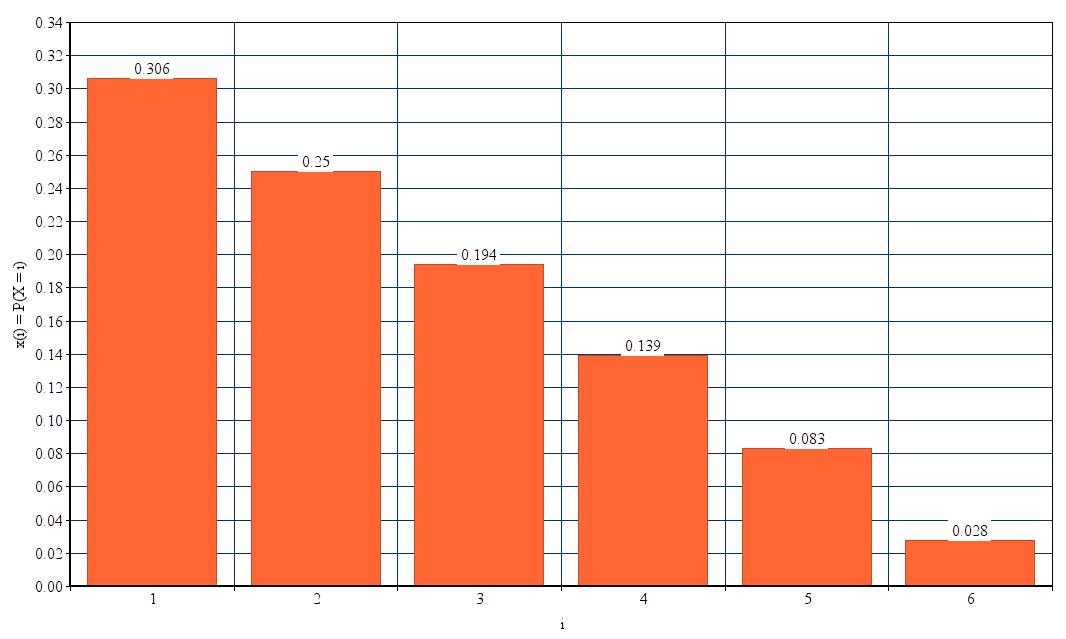
\includegraphics[width=0.8\textwidth]{xminvert}
    \end{figure}
	
	\item Verteilungsfunktion: Die Bestimmung der Verteilungsfunktion fand über Addition der einzelnen Verteilungen statt.\newline
	$A(i) = P(X \leq i) = \sum_{t=0}^i\frac{1 + (2 * (t - 1))}{36} = 
    \begin{cases}
        \frac{11}{36}& \quad \text{wenn } i = 1\\
        \frac{20}{36} & \quad \text{wenn } i = 2\\
        \frac{27}{36} & \quad \text{wenn } i = 3\\
        \frac{32}{36} & \quad \text{wenn } i = 4\\
        \frac{35}{36} & \quad \text{wenn } i = 5\\
        \frac{36}{36} & \quad \text{wenn } i = 6\\
    \end{cases}
    $ \\
    \begin{figure}[!htbp]
      \centering
        \caption{Zeichnung der Verteilungfunktion}
        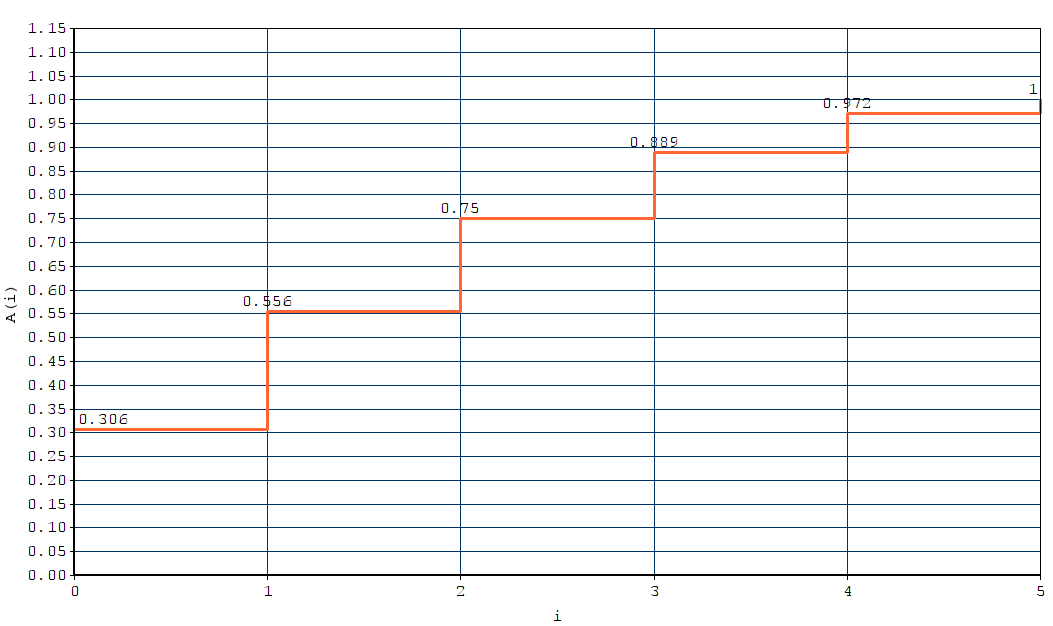
\includegraphics[width=0.8\textwidth]{xminvertfkt}
    \end{figure}
	
	\item Erwartungswert: $E[X] = m_1 = \sum_{i}i * x(i) = \sum_{i}i * \frac{1 + (2 * (i - 1))}{36} = 1 * \frac{11}{36} + 2 * \frac{9}{36} + 3 * \frac{7}{36} + 4 * \frac{5}{36} + 5 * \frac{3}{36} + 6 * \frac{1}{36} = \frac{91}{36} \approx 2,53$\newline
    \item Varianz: $E[X^2] = m_2 = \sum_{i}i^2 * x(i) = \sum_{i}i^2 * \frac{1 + (2 * (i - 1))}{36} = 1^2 * \frac{11}{36} + 2^2 * \frac{9}{36} + 3^2 * \frac{7}{36} + 4^2 * \frac{5}{36} + 5^2 * \frac{3}{36} + 6^2 * \frac{1}{36} = \frac{301}{36} \approx 8.36$
    \\
    $VAR[X] = m_2 - m_1^2 = \frac{301}{36} - (\frac{91}{36})^2 \approx 1,97$ 
\end{enumerate}

\subsubsection*{$X_{max}$:}

\begin{enumerate}
	\item Wertebereich: X hat diskreten Wertebereich mit $X \in \{1, \dots, 6 \}$
	\item Verteilung: Die Bestimmung der Verteilung fand über die Bestimmung aller Möglichkeiten für jede Augenzahl von $\{1, \dots, 6 \}$ statt und sieht folgendermaßen aus:\newline
	$x(1) = P(1) = \frac{m_i}{m} = \frac{1}{6^2} = \frac{1}{36}$,\newline
	$x(2) = \frac{3}{36}$, $x(3) = \frac{5}{36}$, $x(4) = \frac{7}{36}$, $x(5) = \frac{9}{36}$, $x(6) = \frac{11}{36}$. 
	
	\begin{figure}[!htbp]
		\centering
		\caption{Zeichnung der Verteilung}
		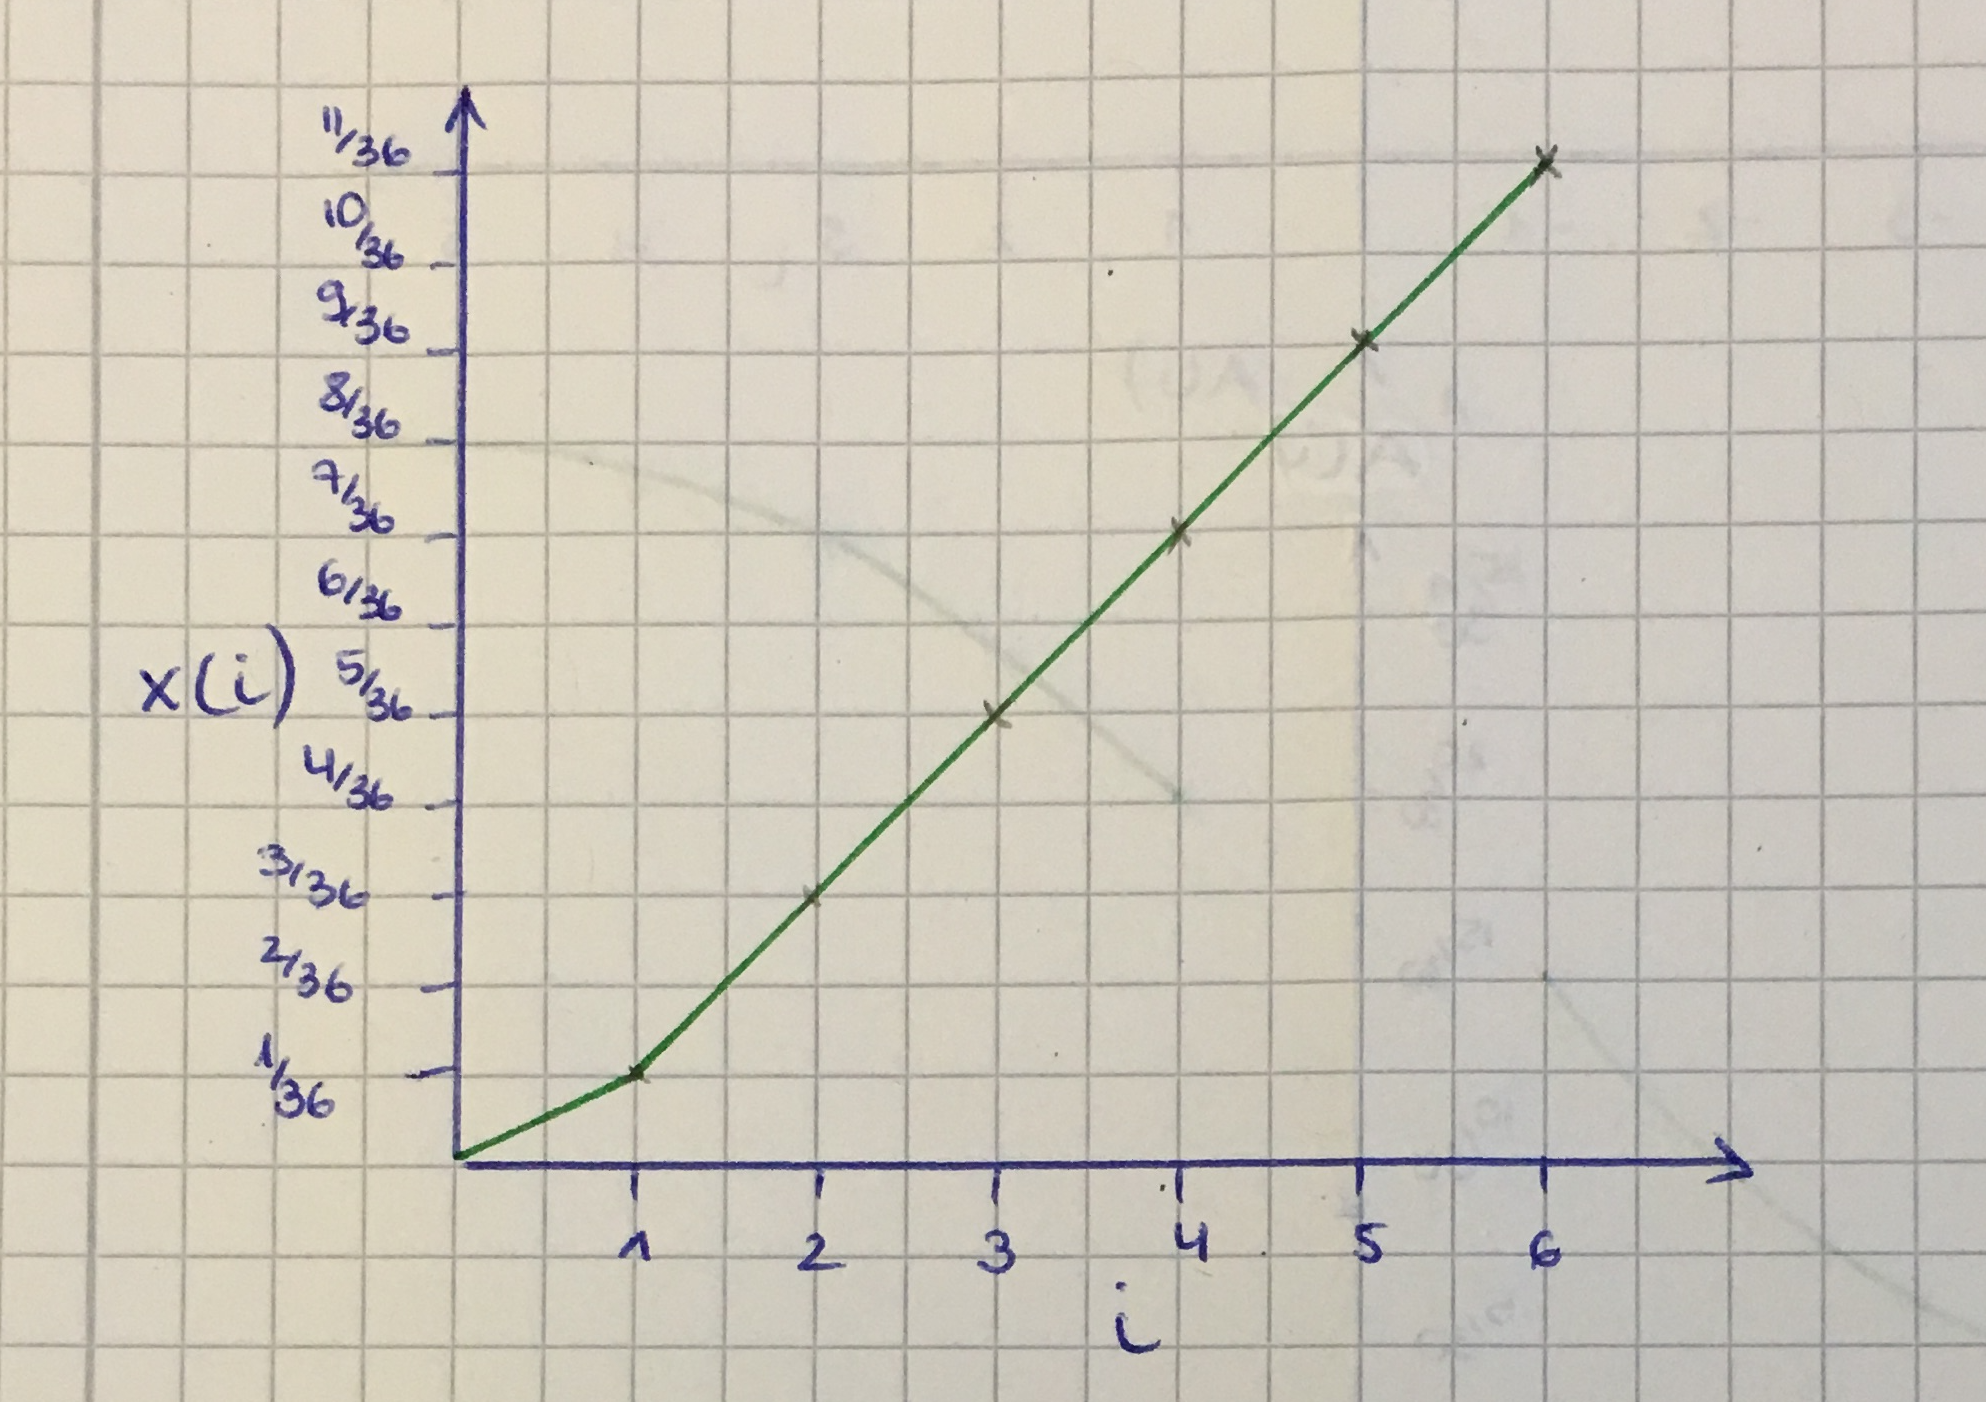
\includegraphics[width=0.8\textwidth]{X_max1.png}
	\end{figure}
	
	\item Verteilungsfunktion: Die Bestimmung der Verteilungsfunktion fand über Addition der einzelnen Verteilungen statt.\newline
	$A(1) = P(A \leq 1) = P(1) = \frac{1}{36}$,\newline
	$A(2) = \frac{4}{36}$, $A(3) = \frac{9}{36}$, $A(4) = \frac{16}{36}$, $A(5) = \frac{25}{36}$, $A(6) = \frac{36}{36} = 1$. 
	
	\item Erwartungswert: $E[X] = m_1 = \sum_{i} i * x(i) = 1 * \frac{1}{36} + 2 * \frac{3}{36} + 3 * \frac{5}{36} + 4 * \frac{7}{36} + 5 * \frac{9}{36} + 6 * \frac{11}{36} \approx 4.472$.
	\item Varianz: $VAR[X] = m_2 + m_1^2$\newline
	$m_2 = E[X^2] = \sum_{i} i^2 * x(i) = 1 * \frac{1}{36} + 4 * \frac{3}{36} + 9 * \frac{5}{36} + 16 * \frac{7}{36} + 25 * \frac{9}{36} + 36 * \frac{11}{36} \approx 21.972$.\newline
	$\rightarrow VAR[X] = 21.972 - (4.472)^2 = 1.982$.
\end{enumerate}

\subsubsection*{$X_{diff_1}$:}

\begin{enumerate}
	\item Wertebereich: X hat diskreten Wertebereich mit $X \in \{0, \dots, 5 \}$
	\item Verteilung: Die Bestimmung der Verteilung fand über die Bestimmung aller Möglichkeiten für jede Summe von $\{0, \dots, 5 \}$ statt und sieht folgendermaßen aus:\newline
	$x(i) =
    \begin{cases}
        \frac{6}{36} = \frac{1}{6} & \quad \text{wenn } i = 0\\
        \frac{10}{36} = \frac{5}{18} & \quad \text{wenn } i = 1\\
        \frac{8}{36} = \frac{2}{9} & \quad \text{wenn } i = 2\\
        \frac{6}{36} = \frac{1}{6} & \quad \text{wenn } i = 3\\
        \frac{4}{36} = \frac{1}{9} & \quad \text{wenn } i = 4\\
        \frac{2}{36} = \frac{1}{18} & \quad \text{wenn } i = 5\\
    \end{cases}
    $
    \\
    oder 
    \\
    $x(i) =
    \begin{cases}
        \frac{1}{6} & \quad \text{wenn } i = 0\\
        \frac{2 * (6 - i)}{36} & \quad \text{sonst }
    \end{cases}
    $ \\
     
    \begin{figure}[!htbp]
      \centering
        \caption{Zeichnung der Verteilung}
        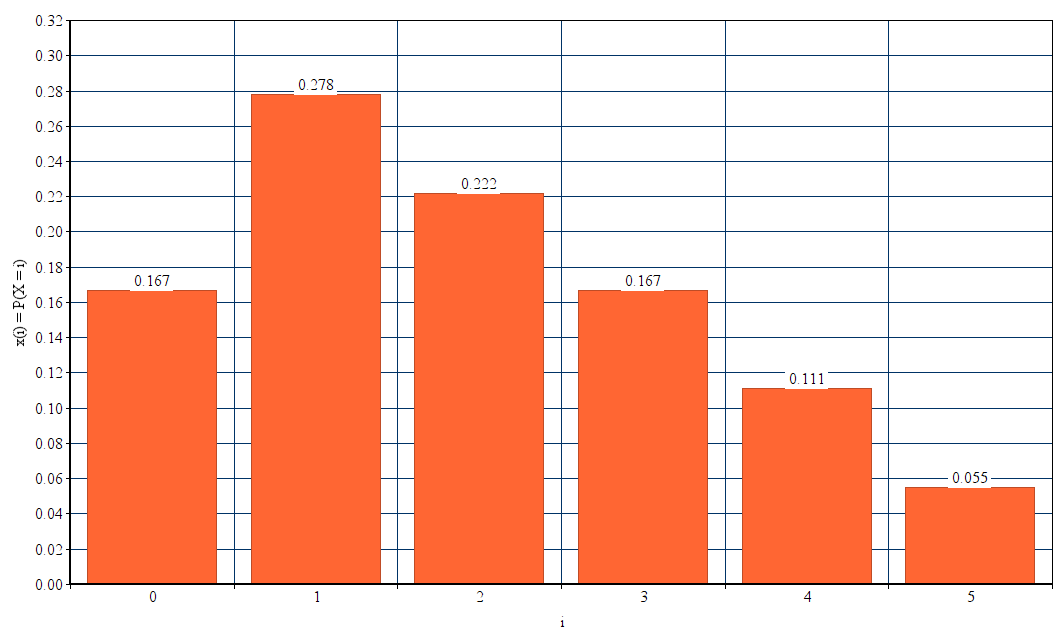
\includegraphics[width=0.8\textwidth]{xdiff1vert}
    \end{figure}
	
	\item Verteilungsfunktion: Die Bestimmung der Verteilungsfunktion fand über Addition der einzelnen Verteilungen statt.\newline
	$A(i) = P(X \leq i) = 
    \begin{cases}
        \frac{6}{36}& \quad \text{wenn } i = 0\\
        \frac{16}{36} & \quad \text{wenn } i = 1\\
        \frac{24}{36} & \quad \text{wenn } i = 2\\
        \frac{30}{36} & \quad \text{wenn } i = 3\\
        \frac{34}{36} & \quad \text{wenn } i = 4\\
        \frac{36}{36} & \quad \text{wenn } i = 5\\
        0 & \quad \text{sonst}
    \end{cases}
    $
    \begin{figure}[!htbp]
      \centering
        \caption{Zeichnung der Verteilungfunktion}
        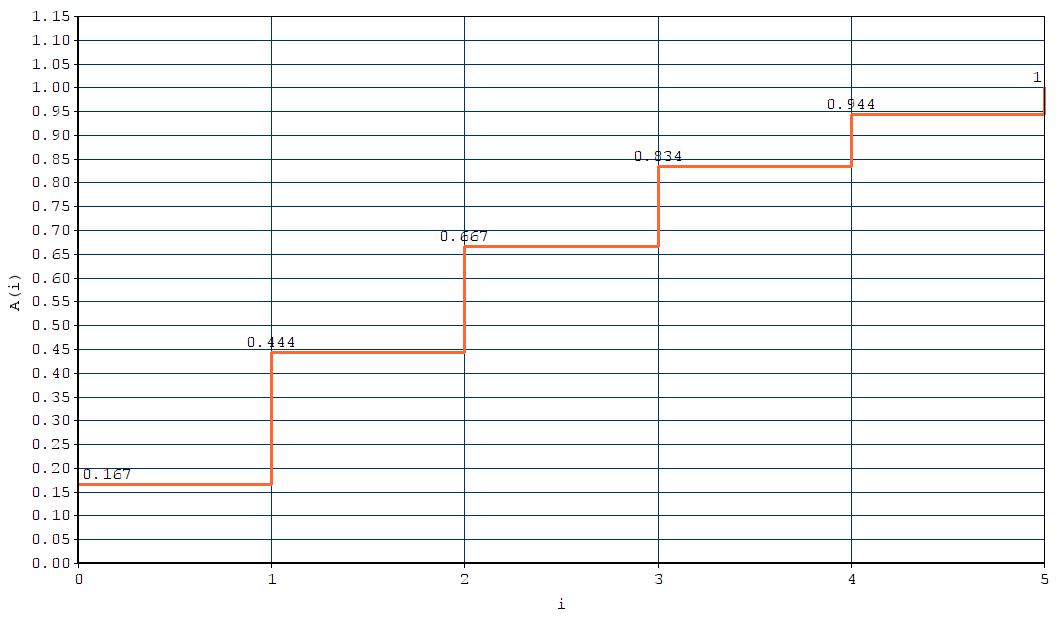
\includegraphics[width=0.8\textwidth]{xdiff1vertfkt}
    \end{figure}
	
	\item Erwartungswert: $E[X] = m_1 = \sum_{i}i * x(i) = \sum_{i}i * = 0 * \frac{6}{36} + 1 * \frac{10}{36} + 2 * \frac{8}{36} + 3 * \frac{6}{36} + 4 * \frac{4}{36} + 5 * \frac{2}{36} = \frac{35}{18} \approx 1,94$.
	\item Varianz: $VAR[X] = m_2 + m_1^2$\newline
	$E[X^2] = m_2 = \sum_{i}i^2 * x(i) = 0^2 * \frac{6}{36} + 1^2 * \frac{10}{36} + 2^2 * \frac{8}{36} + 3^2 * \frac{6}{36} + 4^2 * \frac{4}{36} + 5^2 * \frac{2}{36} = \frac{35}{6} \approx 5,83$
    \\
    $VAR[X] = m_2 - m_1^2 = \frac{35}{6} - (\frac{35}{18})^2 \approx 2,05$ .
\end{enumerate}

\subsubsection*{$X_{diff_2}$:}

\begin{enumerate}
	\item Wertebereich: X hat diskreten Wertebereich mit $X \in \{-5, \dots, 5 \} \backslash \{0\}$
	\item Verteilung: Die Bestimmung der Verteilung fand über die Bestimmung aller Möglichkeiten für jede Differenz von $\{-5, \dots, 5 \} \backslash \{0\}$ statt und sieht folgendermaßen aus:\newline
	$x(-5) = P(-5) = \frac{m_i}{m} = \frac{1}{6^2 - 6} = \frac{1}{30}$,\newline
	$x(-4) = \frac{2}{30}$, $x(-3) = \frac{3}{30}$, $x(-2) = \frac{4}{30}$, $x(-1) = \frac{5}{30}$, $x(1) = \frac{5}{30}$, $x(2) = \frac{4}{30}$, $x(3) = \frac{3}{30}$, $x(2) = \frac{2}{30}$, $x(1) = \frac{1}{30}$. 
	
	\begin{figure}[!htbp]
		\centering
		\caption{Zeichnung der Verteilung}
		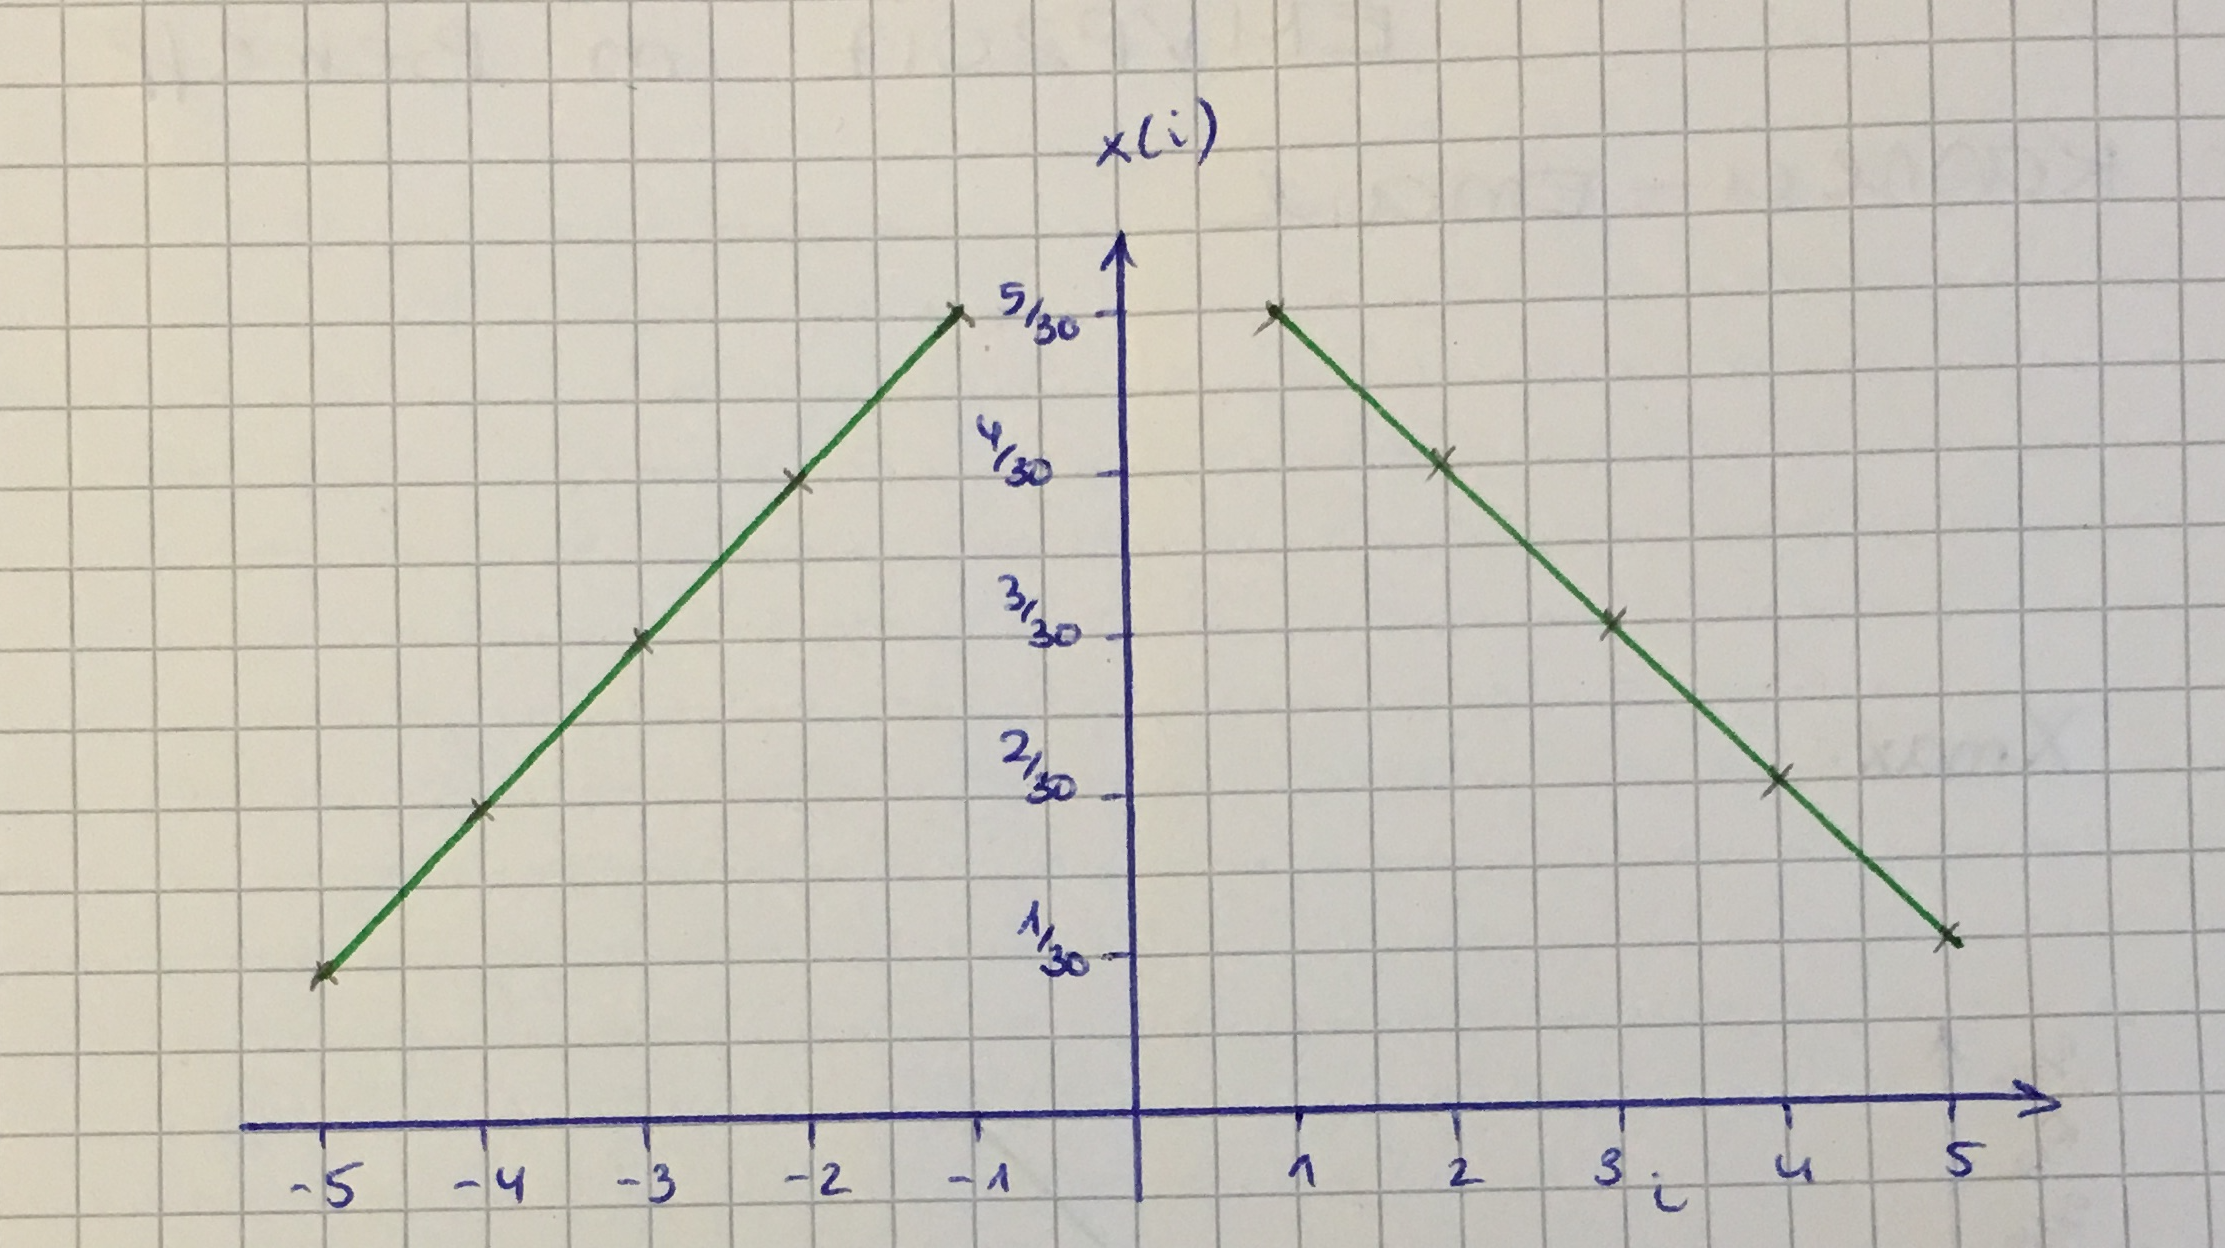
\includegraphics[width=0.8\textwidth]{X_diff1.png}
	\end{figure} 
	
	\item Verteilungsfunktion: Die Bestimmung der Verteilungsfunktion fand über Addition der einzelnen Verteilungen statt.\newline
	$A(-5) = P(A \leq -5) = P(-5) = \frac{1}{30}$,\newline
	$A(-4) = \frac{3}{30}$, $A(-3) = \frac{6}{30}$, $A(-2) = \frac{10}{30}$, $A(-1) = \frac{15}{30}$, $A(1) = \frac{20}{30}$, $A(2) = \frac{24}{30}$, $A(3) = \frac{27}{30}$, $A(4) = \frac{29}{30}$, $A(1) = \frac{30}{30} = 1$. Zeichnung der Verteilungsfunktion: 
	
	\item Erwartungswert: $E[X] = m_1 = \sum_{i} i * x(i)$. Da sich die einzelnen Summanden in der Berechnung des Erwartungswertes gegenseitig aufheben, ist $E[X] = 0$.
	\item Varianz: $VAR[X] = m_2 + m_1^2$\newline
	$m_2 = E[X^2] = \sum_{i} i^2 * x(i) = 25 * \frac{1}{30} * 2 + 16 * \frac{2}{30} * 2 + 9 * \frac{3}{30} * 2 + 4 * \frac{4}{30} * 2 + 1 * \frac{5}{30} * 2 = 7$.\newline
	$\rightarrow VAR[X] = 7 - 0^2 = 7$.
\end{enumerate}

\subsection*{Aufgabe 3}

\begin{itemize}
	\item[a.)] Wertebereich: $X$ hat den Wertebereich mit $X \in \{1, \dots, \infty \}$.
	\item[b.)] Die Zufallsvariable $X$ ist nach der geometrischen Verteilung verteilt, allerdings mit einer kleinen Abwandlung: In dem Skript der Vorlesung beschreibt die Zufallsvariable $X$ die Anzahl der Fehlversuche bis zu einem gewünschten Erfolg, in der Aufgabe beschreibt die Zufallsvariable $X$ jedoch die Anzahl aller Würfe bis zum gewünschten Erfolg, also im Allgemeinen immer einen Wurf mehr. Die Verteilungsfunktion für $X$ lautet dann: $P(X \leq t) = p * \sum_{i}^{t} (1-p)^{i-1}$, wobei $t$ das Ereignis ist, das maximal auftritt, $p$ die Erfolgswahrscheinlichkeit und $i$ die Zählvariable bis $t$. 
	\item[c.)] Wahrscheinlichkeit höchstens 4 Würfe bis 6 zu brauchen:\newline
	$P(X \leq 4) = \frac{1}{6} * \sum_{i = 1}^{4} (\frac{5}{6})^{i-1} = \frac{1}{6} * ( \frac{5}{6}^0 + \frac{5}{6}^1 + \frac{5}{6}^2 + \frac{5}{6}^3) \approx 0.52 \rightarrow 52\%$.
\end{itemize}

\section*{Problem 1.2}

\subsection*{Aufgabe 1}

\begin{figure}[!htbp]
  \centering
    \caption{Verteilungsfunktionen von geometrischer und Verteilungsdichtefunktion exponentieller Verteilung}
    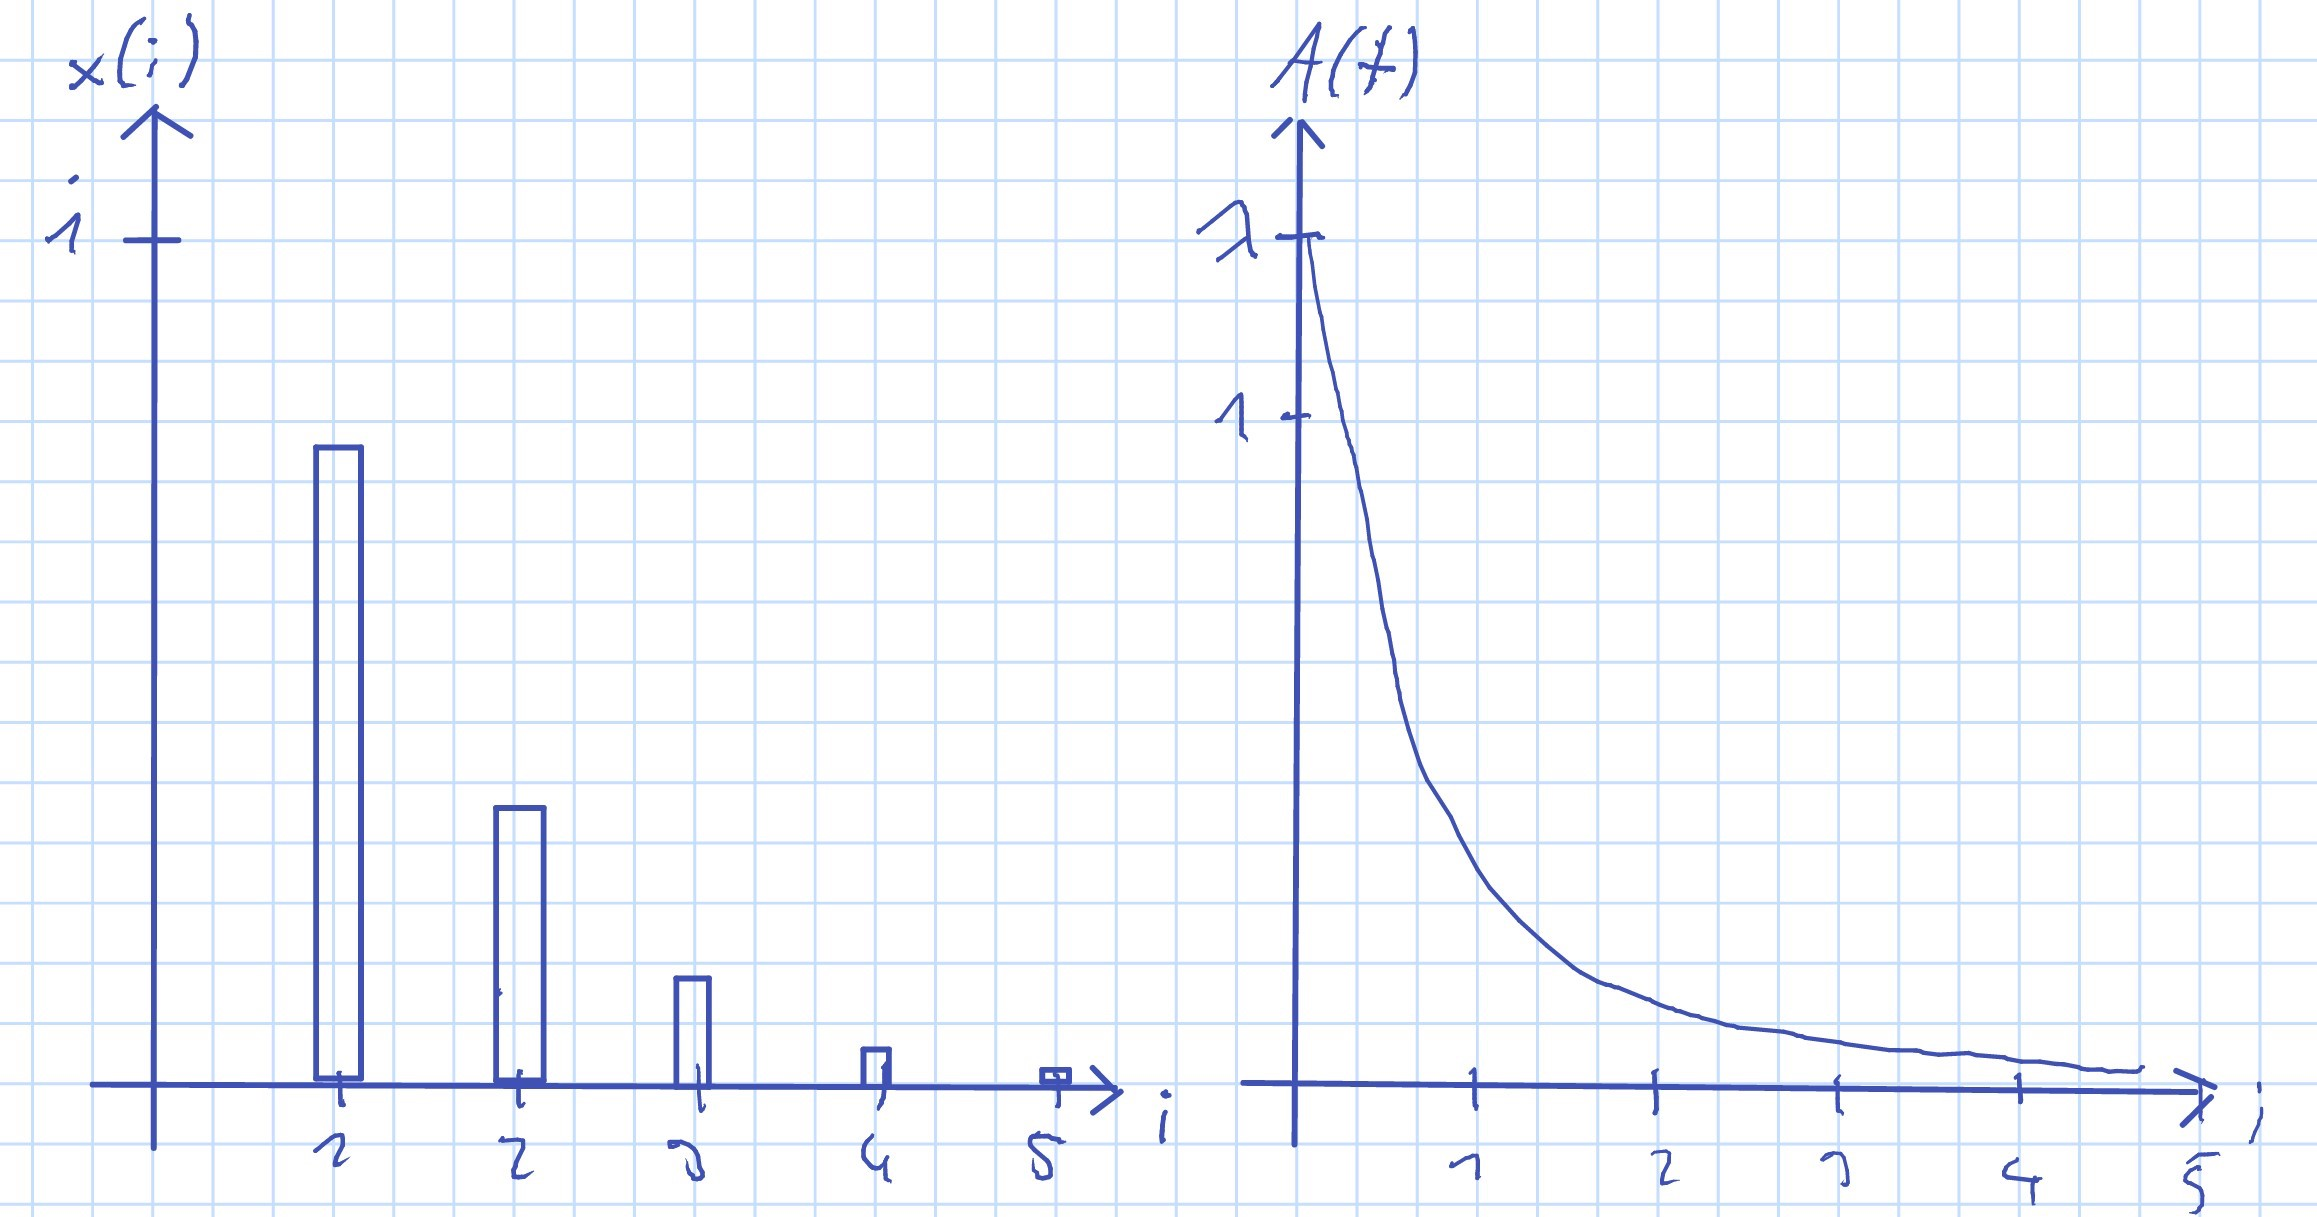
\includegraphics[width=0.8\textwidth]{a4vert}
\end{figure}
Hauptunterschied: Während bei der diskreten geometrischen Verteilung sogenannte Sprünge (diskrete Schritte) in der Verteilungsfunktion erkennbar sind, ist die Verteilungsfunktion der exponentiellen Verteilung eine geglättete kontinuierliche Kurve. 
\newpage
\subsection*{Aufgabe 2}
     
\begin{figure}[!htbp]
  \centering
    \caption{Verteilung der geometrischen Verteilung und Verteilungsfunktion der exponentiellen Verteilung}
    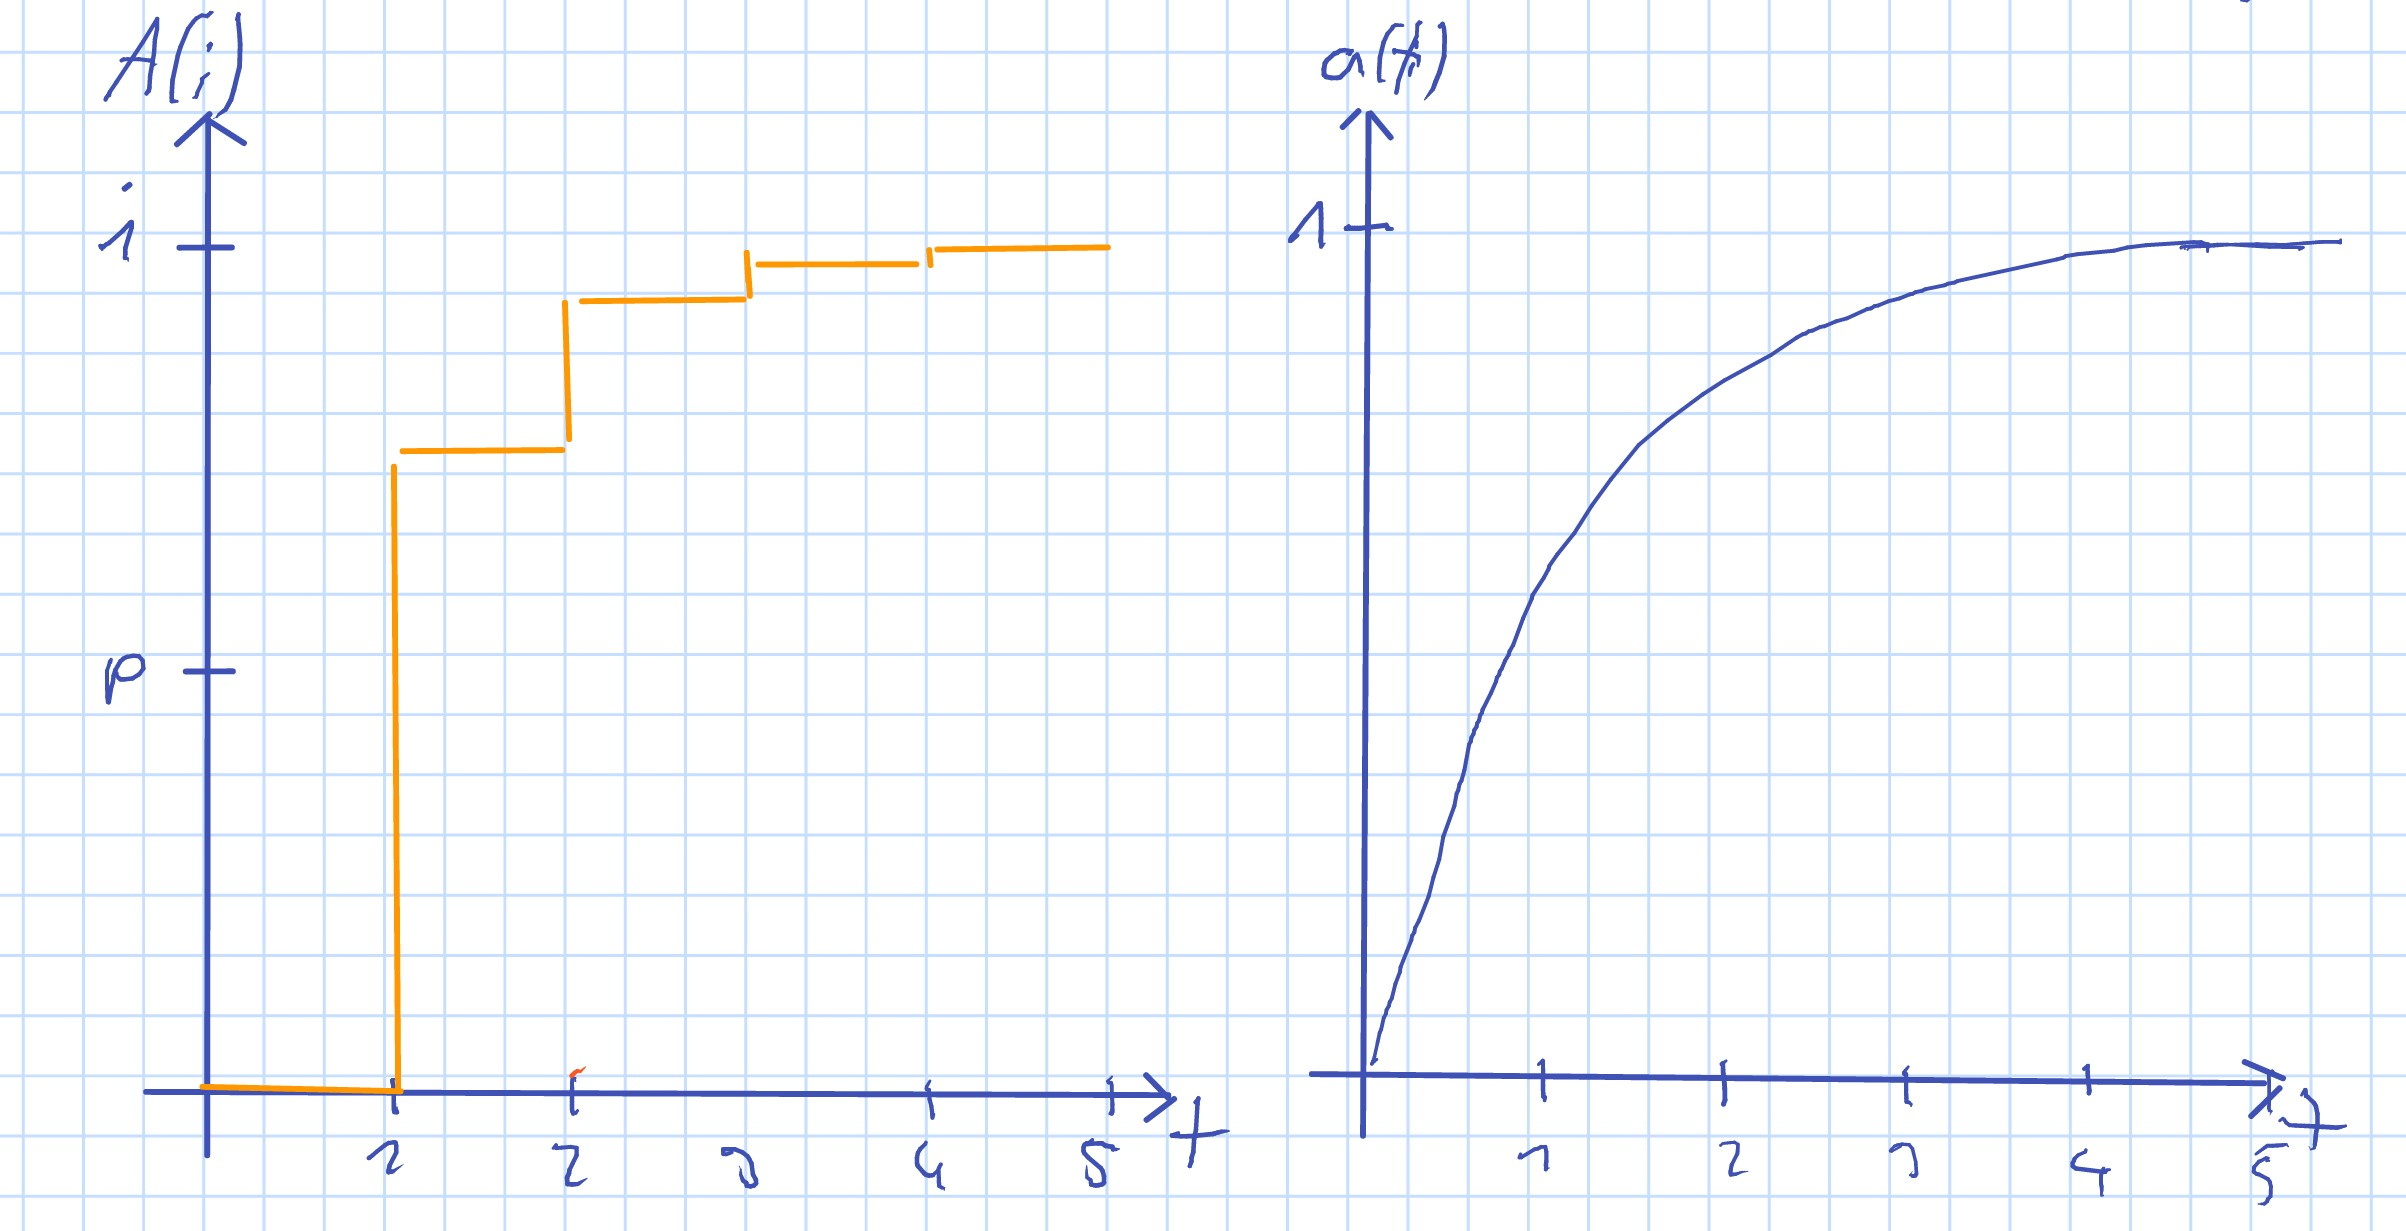
\includegraphics[width=0.8\textwidth]{a4vertfkt}
\end{figure}
Hauptunterschied: Bei der exponentiellen Verteilung kann man den Wert der Verteilungsfunktion nicht direkt an der Kurve ablesen, sondern muss dafür das Integral berechnen. Bei der geometrischen Verteilung hingegen kann man den Wert der Verteilungsfunktion direkt an der Kurve ablesen. 

\subsection*{Aufgabe 3}

Wahrscheinlichkeit für $P(X \leq 1)$ bei der geometrischen Verteilung:\newline
$P(X \leq 1) = p * \sum_{i = 1}^{1} (1-p)^i = p * (1-p) = p - p^2$.\newline

Wahrscheinlichkeit für $P(X \leq 1)$ bei der exponentiellen Verteilung:\newline
$P(X \leq 1) = \int_{0}^{1} a(\tau) d\tau = [a(t)]_0^1 = [\lambda * e^{-\lambda} * t]_0^1 = A(1) - A(0) = (1 - e^{-\lambda * 1}) - (1 - e^{-\lambda * 0}) = 1 - e^{-\lambda} - 1 + 1 = 1 - e^{- \lambda}$ 


\end{document}